\documentclass[nofonts,nobib]{tufte-handout}

%% Font Stuff
\usepackage{fontspec}
\usepackage{ifxetex}
% \fontspec{EB Garamond}
\setmainfont[Ligatures=TeX,Mapping=tex-text,Numbers=OldStyle]{EB Garamond}
\setsansfont{Noto Sans}
\setmonofont{EB Garamond}
\usepackage{booktabs}
\usepackage{lipsum}
% a new font family for different languages
\newfontfamily\myfont[]{Noto Sans CJK JP}
\newfontfamily\symbolfont[]{Noto Sans Symbols}

\ifxetex
  \newcommand{\textls}[2][5]{%
    \begingroup\addfontfeatures{LetterSpace=#1}#2\endgroup
  }
  \renewcommand{\allcapsspacing}[1]{\textls[15]{#1}}
  \renewcommand{\smallcapsspacing}[1]{\textls[10]{#1}}
  \renewcommand{\allcaps}[1]{\textls[15]{\MakeTextUppercase{#1}}}
  \renewcommand{\smallcaps}[1]{\smallcapsspacing{\scshape\MakeTextLowercase{#1}}}
  \renewcommand{\textsc}[1]{\smallcapsspacing{\textsmallcaps{#1}}}
\fi

\usepackage[backend=biber,autocite=footnote]{biblatex-chicago}
\addbibresource{bibliography.bib}
% % % \DefineBibliographyStrings{english}{%
% %   references = {Works Cited},
% % }
\renewcommand{\cite}[2][0pt]{%
  \sidenote[][#1]{\fullcite{#2}}%
  }

%   wrapfig
\usepackage{wrapfig}

\title{Watch the Tiger Walk: Another Study in Intention}
\author{Rachael Carlson}
\date{\today}
\begin{document}
\maketitle

\section{Introduction}
The twenty-first century musician is faced with a dilemma. The future of the existence of the professional musician is uncertain. The consumption of music seems to be at all-time highs and yet previous sources of income are unreliable: the musician is no longer able to rely on income from album sales, radio play and other royalties, sheet music sales, or patronage. The twenty-first century musicians appears to require all of these sources in order to make a living as a professional musician. In addition to these sources of income, the musician will need to find income from performances, instruction, YouTube and other internet streaming services royalties, and commissions from publications and magazines. \\

The finger-style guitarist is not immune to these changes. In some cases, the finger-style guitarist is at the forefront of these changes, a harbinger of the future. One of the earliest YouTube celebrities was Andy McKee. This article will attempt to discern how musicians are surviving, or even thriving, by examining their apparent revenue streams. It will have three goals. First, to examine the available methods of consuming a twenty-first century musician's output. The aim for this examination is to establish a baseline by which one can measure one's own progress in relation to those who have achieved notoriety before him or her. The focus of this research will primarily be on finger-style guitarists.  Second, to examine ``Watch the Tiger Walk,'' an original composition, as a case study in which the means examined in the first portion are fully or partially enacted for a single composition. I will begin the necessary work on a transcription and I will produce audio and video.  Third, I will begin work on reinforcing my website in preparation for a life as a professional musician and finger-style guitarist.

\section{Internet Presence}
\label{sec:internet-presence}
There are numerous ways in which a twenty-first century musician supports him or herself. The most visible component of this support is the internet. A musician is judged upon his or her social presence on the internet.

\subsection{The Data}
\label{sec:data}
The parameters for the research are as follows: finger-style guitarist, a website, some level of notoriety. I also gave consideration to whether the artist is established or up-and-coming, ultimately deciding to focus roughly half of each group. 41 artist websites were analyzed. 21 artists could be considered up-and-coming and 20 could be considered established. The original intention was to include artists outside of the finger-style sphere, however, the data set quickly became too immense and it was necessary to exclude artists outside of finger-style guitar. It may be beneficial in the future to take a more inclusive approach to this research in order to better inform the reader. A concerted effort was made to include musicians outside of the United States. There appears to be a tendency among burgeoning artists to rely on Facebook to share their craft.

Through an analysis of a subsample of the data, 26 codes were developed. The codes were carefully selected to demonstrate important elements of an artist's website. The codes fell into roughly four categories: persona, display, technologies, and commerce. These codes range from the manner in which the artist attested to his or her legitimacy to the type of Content Management System (\textsc{cms}) that the artist uses.

This data is a snapshot of the immense world of finger-style guitar as it exists on the internet. The rapid changes in technology may deem this essay obsolete quite soon. This data set has been included in the appendix.
%   \begin{table*}\centering
%     \small
%     \begin{tabular}{l l}\toprule
%       Artist  &  \\\midrule
%       Title & \emph{Garamond Premier Pro} Display Italic 28pt\\
%       Tuning & \emph{EB Garamond} 12 Regular 10pt\\
%       Octave Designation & \emph{EB Garamond} 12 Regular 10pt subscript\\
%       Composer & \emph{EB Garamond} 12 Regular 10pt\\
%       Clef & \emph{Adobe Garamond Pro} Bold 11pt\\
%       Noteheads & \emph{Noto Sans} Regular 12pt\\
%       Left-Hand Fingering & \emph{Noto Sans} Symbols 12pt\\
%       Right-Hand Fingering & \emph{EB Garamond} 08 Regular 8pt\\
%       Copyright and Page Numbers & \emph{EB Garamond} 08 Regular 8pt\\
%       \bottomrule
%   \end{tabular}
%   \caption{DESCRIBE THE DATA IN AN INTELLIGENT MANNER. Each artist's
%   website is listed in the References section.}
% \end{table*}
\subsection{Analysis}
\label{sec:analysis}

There were several codes which fall into a subjective field of determination. These were the claims to legitimacy, visual display, and the openness of the artist to his or her craft. The content of these codes was based upon
\begin{table}
  \centering
  \small
  \begin{tabular}{p{0.27\linewidth}p{0.15\linewidth}p{0.45\linewidth}}\toprule
    Claim to Legitimacy & Number of artists & Description \\\midrule
    Associative & 1 & artists with whom artist associates \\
    Freshness & 1 & a new face in the finger-style scene \\
    Historical & 3 & in the context as an artist \\
    Inspirational & 1 & a story which inspires legitimacy \\
    Instructional & 3 & through their abilities as teachers \\
    Material & 2 & sponsorships or instruments \\
    Musical & 15 & audio and video presentations \\
    No claims & 4 & artist makes no overt claim to legitimacy \\
    Testimonial & 13 & reviews of artist by artists and other entities \\
    Youthfulness & 1 & age of artist is claim to legitimacy \\
      \bottomrule
  \end{tabular}
  \caption{The array of claims to legitimacy.}
\end{table}
the subjective interpretation of the author. A major component of the artists' web sites is how the artist establishes his or her legitimacy as a performer and/or composer. Some artists claimed several different types of legitimacy at the same time. For instance, Pierre Bensusan's web site claims his legitimacy through his musicality and through sponsorships. His sponsorships have been coded as a claim to legitimacy through material means. Another example of an artist claiming legitimacy through material means would be Alex Anderson, who makes a point to associate himself with the harp guitar. Another subject code was the appearance of the artist's web site. All of the artist web sites had pictures of the artist on the landing or home page. Some artists had color schemes which made the text illegible. The different visual displays that are utilized by finger-style guitarists span the last twenty years of graphic design on the internet. Some artists are closed about their art in that they do not display any indication that they are willing to teach someone their craft. Other artists are open about their art. Those that are open are open in different ways. Ewan Dobson and Mike Dawes offer lessons over Skype.
\begin{margintable}\centering
  \small
  \begin{tabular}{p{0.4\textwidth} l l}\toprule
    Question & yes & no \\\midrule
    mobile-friendly? & 22 & 19\\
    Adobe Flash? & 4 & 37\\
    https? & 7 & 34\\
    streaming audio? & 20 & 21\\
    streaming video? & 35 & 6\\
    booking? & 31 & 10\\
    Twitter feed? & 4 & 37\\
    electronic newsletter? & 19 & 22\\
    \bottomrule
  \end{tabular}
  \vspace{6pt}
  \caption{Yes-or-no questions asked of the artists' websites.}
\end{margintable}

Several questions, ranging from visual to technical, were coded for each web site. While it may have seemed arbitrary at first to ask some of the questions listed in Table 2, the responses can be quite surprising. For instance, a little under half of the web sites were not friendly to mobile browsers. This is perhaps indicative of a lag between changes in the display of finger-style guitarists' web sites and worldwide trends in internet browsing. As seen in Figure 1, around October of 2016, the market share of mobile browsers surpassed that of desktop browsers. It may be wise for all finger-style guitarists, as well as content producers in general, to recognize the importance of creating an adequate user experience for the mobile platform.
\begin{figure}
  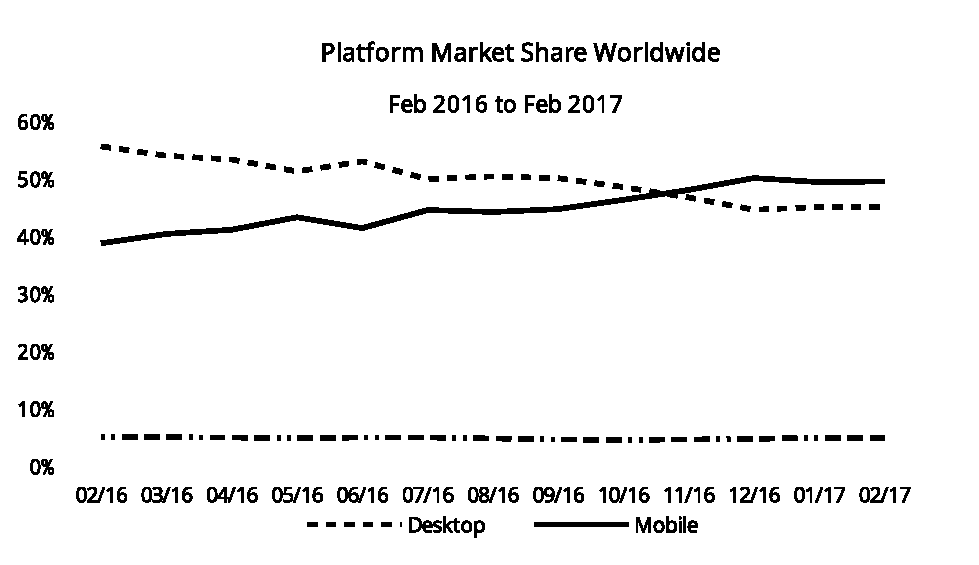
\includegraphics[width=1.00\textwidth]{platformMarketShare.eps}
  \caption{The distribution of platforms from around the world which browsed the
    internet from February, 2016 to February 2017. \fullcite{statCounter1}}
  \label{fig:StatCounter1}
\end{figure}
\begin{figure}
  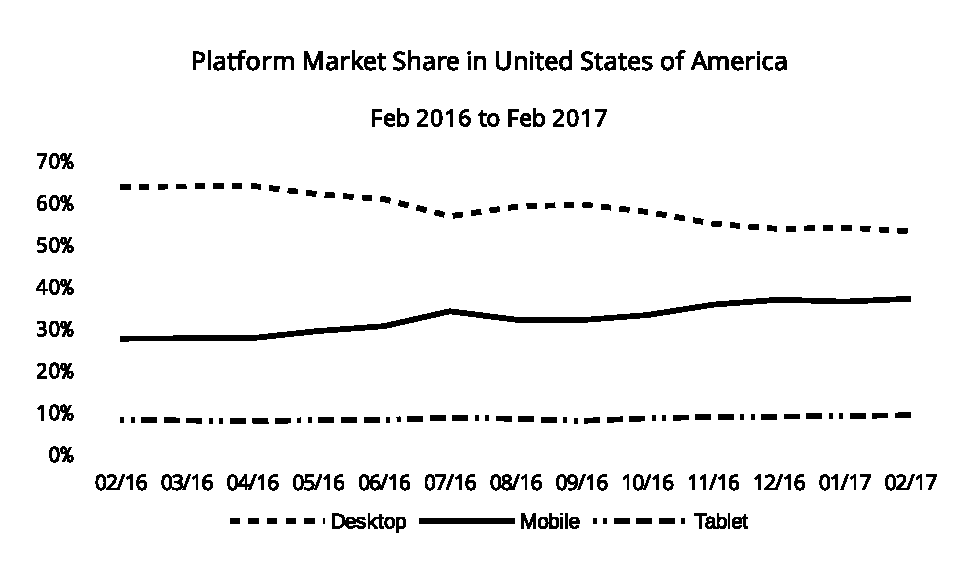
\includegraphics[width=1.00\textwidth]{platformMarketShareUS.eps}
  \caption{The distribution of platforms from the United States of America which browsed the
    internet from February, 2016 to February 2017. \fullcite{statCounter2}}
  \label{fig:StatCounter2}
\end{figure}
The result of not making one's web site friendly to mobile users is lessened when one examines the market share for only the United States of America, seen in Figure 2. Four web sites require Adobe Flash in order to experience content. These four web sites are leaving at least half of the users of the internet in the dark as Adobe has discontinued Flash development for mobile platforms.\autocite{adobeFlash} It is also quite surprising that only half of the artists have streaming audio on their web sites while every artist except six have streaming video. This may be an indication of the near-ubiquity of streaming video on the internet. It would have been interesting to see the shift from streaming audio to streaming video in the 2000s. \emph{Internet Archive}'s ``WaybackMachine'' may be a way in which to examine the developments of finger-style guitarists' web sites through the years.\autocite{internetArchive}
\begin{margintable}\centering
  \small
  \begin{tabular}{l l}\toprule
    \textsc{cms} & Number\\\midrule
    Bandzoogle & 4\\
    Hostbaby & 2\\
    Joomla & 1\\
    JuanPaSystems & 1\\
    ProdgWeb & 1\\
    Squarespace & 7\\
    Sumo & 1\\
    Truefire & 1\\
    WebsiteBuilder & 1\\
    Wix & 3\\
    Wordpress & 1\\\midrule
    Total & 23\\
    \bottomrule
  \end{tabular}
  \vspace{6pt}  
  \caption{Distribution of discernable Content Management Systems among the
    web sites of finger-style guitarists.} 
\end{margintable}
An area of particular interest to me was the manner in which these web sites managed their content. I was able to determine the Content Management Systems (\textsc{cms}) of 23 sites as seen in Table 3. The most represented \textsc{cms} is Squarespace with 7 artists followed by Bandzoogle at 4 and Wix at 3. I find this interesting because some of these \textsc{cms}'s integrate components into their systems which may assist an artist in the management of his or her web site. For instance, Bandzoogle assists in creating mobile-friendly web sites with a web store, newsletters, streaming services, blogs, and a gig calendar.\cite[12pt]{bandzoogle} The web sites which did not have any discernible manner in which to determine content creation may or may not have been created and managed with a \textsc{cms}.

One of the primary catalysts for this essay was to conduct a review of the distribution of sheet music within a digital finger-style domain. Almost every web site delivered their transcriptions in a different way. A few sites, such as Pierre Bensusans' had what appeared to be a custom built store. Others, such as Gareth Pearson, linked out to other venues such as CandyRat or Bandcamp. Many artists sold their products through PayPal in which the site redirected the customer to PayPal to make his or her purchase. Several sites, including Alex de Grassi's, delivered through a storefront created by their \textsc{cms}.

Each difference in the delivery of content can either enhance or detract from the user experience. This essay is only a survey, not a discussion, of expected graphical design components of a finger-style guitarist's web site.
\section{Transcription}
A distinguishing characteristic of the finger-style guitarist's website is a section of sheet music, scores, or transcriptions of the artist's works. This seems to be a unique component of the finger-style culture. Sadly, while the transcriptions are becoming marginally better than ascii-tab on the internet, the quality of the transcriptions produced by these musicians is not on par with the quality of playing or composition. This could be attributed to different factors, all of which are for another essay. Here I will discuss near-best practices for the production of finger-style transcriptions.
\subsection{Methods}
\label{sec:methods}
The primary method espoused by John Stropes of Stropes Editions, Ltd. is a double-impression method utilizing Finale and Adobe InDesign. The methods used in this document are as follows: XeLaTeX for the typesetting of this essay and the same double-impression method of Finale and Adobe InDesign used by Stropes Editions for the transcription. I also used FontForge to modify some of the fonts that are used in Finale.

\subsection{Typography}
\label{sec:typography}
Stropes Editions, Ltd. has been at the forefront of the development of transcription and typesetting for finger-style guitar since the 1980s. These developments can be examined from a historical perspective starting with \emph{Twentieth Century Masters of Finger-Style Guitar}, \emph{Leo Kottke: Eight Songs}, and \emph{Michael Hedges: Rhythm, Sonority, Silence} to ``Ants'' and the unreleased grid notation for ``Madness.'' These examples represent pinnacles n the art of sheet music engraving for the guitar.  Due to these innovations, it can be difficult to reach beyond the conventions established. When the transcriptions from Stropes Editions are examined within a historical context one is able to tell that there is a sense that innovation is more important than tradition. 
% I am reminded of a quote by the highly influential designer, Paul Rand, ``new becomes threatening, the old reassuring.''
\begin{figure*}\centering
        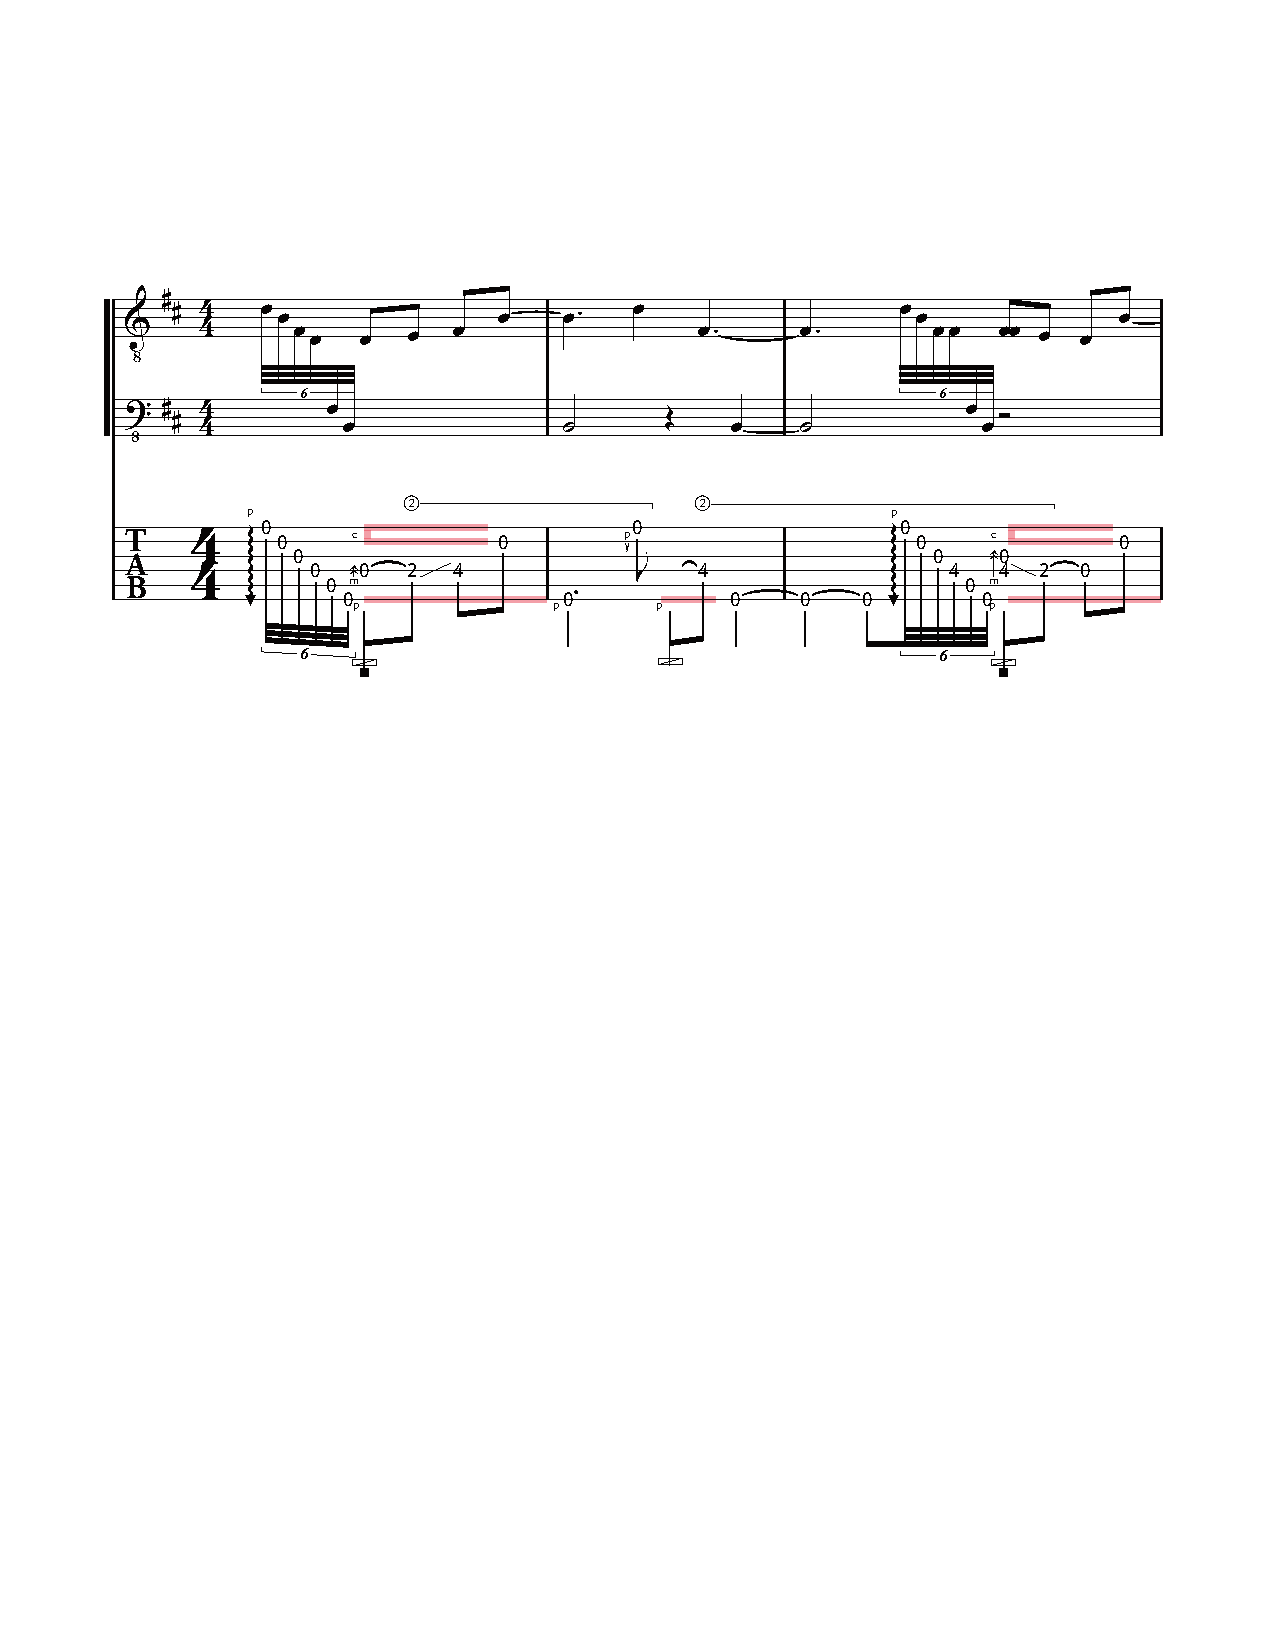
\includegraphics[width=1.00\textwidth]{watchTheTigerWalk20170326.pdf}
    \caption{``Watch the Tiger Walk'' by Rachael Carlson, mm. 1--2.}
    \label{fig:somthing}
  \end{figure*}
The fonts used at Stropes Editions are Helvetica \textsc{lt} Std, \textsc{itc} Franklin Gothic and occasionally Times New Roman. While the design of the \textsc{sel} sheet music would not be considered bad, in fact they stand apart from all previous transcriptions in their beauty, they \emph{have} established themselves as reassuring. It can be quite difficult to produce a score for finger-style guitar which does not either copy \textsc{sel} or fall into the category of ugly music for the guitar. The difficulty of producing a unique voice within the field of music engraving is perhaps due to this feeling of reassurance. We are tasked with the necessity of simultaneously producing documents that are almost audible in their beauty and ensuring the maximum level of legibility. Established music publishers such as Bärenreiter and Henle Verlag may have specific guidelines to produce a base-level of legibility. Perhaps, the requirement of legibility at a specific distance from the page in order to anticipate real-world scenario of music reading.
  
I have carefully chosen the typography of my transcriptions. And while I wish that I could say that I have found the perfect combination, I can not. What I can say, is that the typography that I have chosen for my transcriptions is designed for optimal legibility at small font sizes while ensuring the reader will not confuse one glyph for another.
  \begin{table}\centering
    \small
    \begin{tabular}{l l}\toprule
      Page Content  & Font \\\midrule
      Title & \emph{Garamond Premier Pro} Display Italic 28pt\\
      Tuning & \emph{EB Garamond} 12 Regular 10pt\\
      Octave Designation & \emph{EB Garamond} 12 Regular 10pt subscript\\
      Composer & \emph{EB Garamond} 12 Regular 10pt\\
      Clef & \emph{Adobe Garamond Pro} Bold 11pt\\
      Noteheads & \emph{Noto Sans} Regular 12pt\\
      Left-Hand Fingering & \emph{Noto Sans} Symbols 12pt\\
      Right-Hand Fingering & \emph{EB Garamond} 08 Regular 8pt\\
      Copyright and Page Numbers & \emph{EB Garamond} 08 Regular 8pt\\
      \bottomrule
  \end{tabular}
    \caption{Weights and sizes of fonts used in my transcriptions.}
\end{table}
Fonts that are designed based upon Claude Garamont (c. 1510 -- 1561) and Robert Granjon (1513 -- 1590) speak to me. Both Garamont and Granjon were French type designers and publishers in France. EB Garamond is an open source project directed by Georg Duffner based upon the \emph{Berner specimen}. This specimen does not contain bold examples. As such, neither does EB Garamond. The default numerical figures used in EB Garamond are old-style. Due to this I use Adobe Garamond Pro for titling which contains numbers and for the clef which looks more attractive in a bold typeface. On the complete opposite end of the Garamond spectrum, for the noteheads and the left-hand fingering I use Google's Noto Sans. This font family was designed for the mobile market as a means to ensure that almost all of the more than 128,000 figures in \emph{The Unicode Standard} are present such than when a user is confronted with a glyph they do not see a white box affectionately called a block of tofu.

There must to be a time when one makes a decision knowing all of the positives and negatives associated with that decision. It is at this point that it is more important that one makes \emph{a} decision than whether that decision is the best possible decision. I have vacillated between ten or so different fonts for my transcriptions. The decision of which font combination ensures readability while expressing an individual voice. This is an extremely difficult set of decisions. If I had enough money to purchase fonts I would most likely use \emph{Garamond Premier Pro} from Adobe and \emph{Whitney} from Hoefler \& Company.\autocites{garamondPremier,hoeflerWhitney} I am attracted to \emph{Whitney} in particular due to the presence of the ``Index'' font subset which contains circled numbers and letters --- {\symbolfont① ② ③ ④ Ⓣ}. My attraction to \emph{Garamond Premier Pro} based on the same discussion above about Gararmont and Granjon while \emph{Garamond Premier Pro} is also a massive font family of 34 different fonts each with a different purpose. This versatility is an extremely attractive feature of a font which will be used to set body copy for study notes and the other ancillary elements of professional sheet music.

\section{Conclusions}
\label{sec:conclusions}

There can only be one conclusion to an essay such as this: there is no conclusion. The technologies involved in constructing both web sites and finger-style transcriptions is in a constant state of development. The prevalence of the mobile platform has become near-ubiquitous within the last five years. The manner in which finger-style guitar transcriptions are produced has changed drastically in the last twenty years. The software that is available to produce finger-style guitar transcriptions are at the users fingertips, a mere download away. While this software may not produce professional-grade transcriptions on the same level as an \textsc{sel} transcription, they have helped begin the process of taking guitar tablature out of the dark ages of ascii-tab. It is not possible to conclude how the future of finger-style guitar is going pan out. What \emph{can} be concluded is that it is incredible to be a finger-style guitarist in an age in which finger-style guitar is experiencing a renaissance. There is a distinct possibility that someone I know may come across or benefit greatly from some new technology that cannot be imagined.

\nocite{alexAnderson,alexDeGrassi,andrewWhite,andyMcKee,billyMcLaughlin,adamRafferty,calumGraham,cliveCarroll,craigDAndrea,evaAtmatzidou,ewanDobson,garethPearson,happyTraum,ianEthanCase,janetFeder,jimmyWahlsteen,jonGomm,kakiKing,kellyValleau,kevinHorrigan,leoKottke,lucaStricagnoli,lucasMich,masaakiKishibe,michaelChap,michaelGul,mikeDawes,murielAnders,peppino,peterCiluzzi,peterFinger,pierre,rayMontford,pino,spencerElliot,sunghaJung,thomasLeeb,timSparks,tommyEmmanuel,trevorGH,vickiGenfan}
% \bibliographystyle{chicagoa}
% \bibliography{bibliography}
\printbibliography
\end{document}
%%% Local Variables:
%%% mode: latex
%%% TeX-master: t
%%% End:
